\documentclass[12pt]{article}
\usepackage[english]{babel}
\usepackage[utf8]{inputenc}
\usepackage{amsmath,amssymb}
\usepackage{graphicx}
\usepackage{hyperref}
\usepackage{booktabs}
\usepackage{pgfplots}
\pgfplotsset{compat=1.18}
\usepackage{helvet} % Arial-like font (Helvetica)
\renewcommand{\familydefault}{\sfdefault} % Use sans-serif (Arial/Helvetica)
\usepackage{setspace} % For line spacing
\onehalfspacing % 1.5 line spacing
\usepackage{geometry} % For margins
\geometry{
    left=2.5cm,
    right=2.5cm,
    top=2.5cm,
    bottom=2.5cm
}
\usepackage{ragged2e} % For text justification
\justifying % Justify all text

\title{Brute Force Algorithms for the Dutch Merchant Problem}
\author{}
\date{}

\begin{document}

\maketitle

\begin{abstract}
This document presents the design, implementation, and experimental analysis of three brute force algorithms for solving the Dutch Merchant Problem, corresponding to \textbf{Fase 3} of the project requirements. The algorithms include: pure brute force enumeration, brute force with pruning techniques, and a hybrid approach combining brute force route selection with dynamic programming for transaction optimization. These algorithms serve as exact solution methods for small instances, establishing optimal baselines for comparison with heuristic and approximation algorithms in \textbf{Fase 4}. The optimal solutions found here will be used as benchmarks to evaluate the quality and performance of efficient (non-exact) algorithms in subsequent phases of the project.
\end{abstract}

\section{Introduction}
\label{sec:introduction}

This document corresponds to \textbf{Fase 3: Diseño de Soluciones Algorítmicas} of the project requirements. According to the project specifications, this phase requires designing and implementing a brute force algorithm that finds the optimal solution, which will serve as a baseline for comparing results in small instances.

The Dutch Merchant Problem, as formalized in the previous phase (Fase 2), is an NP-Complete optimization problem \cite{garey1979} that combines routing decisions (which ports to visit and in what order) with transaction optimization (what to buy and sell at each port). The problem is related to the Prize-Collecting Traveling Salesman Problem \cite{MarchettiSpaccamela2007PrizeCollectingTS}, which is known to be NP-hard \cite{karp1972}. Given the computational intractability of the problem for large instances, this phase focuses on developing exact algorithms that can solve small instances optimally.

The purpose of implementing brute force algorithms, as required by Fase 3, is twofold:
\begin{enumerate}
    \item To establish optimal solutions for small instances, which will serve as benchmarks for evaluating the quality of heuristic and approximation algorithms in Fase 4. These optimal solutions are essential for measuring the approximation ratio and solution quality of efficient (non-exact) algorithms.
    \item To empirically demonstrate the exponential growth in computational complexity, providing concrete evidence of the problem's intractability and justifying the need for heuristic approaches in Fase 4.
\end{enumerate}

We present three progressively more efficient approaches:
\begin{itemize}
    \item \textbf{Pure Brute Force}: Exhaustive enumeration of all routes and decision sequences, serving as the baseline optimal algorithm.
    \item \textbf{Brute Force with Pruning}: Same enumeration strategy enhanced with backtracking and feasibility pruning to eliminate infeasible branches early.
    \item \textbf{Hybrid (Brute Force + Dynamic Programming)}: Separates route selection (brute force) from transaction optimization (dynamic programming), achieving significant performance improvements while maintaining optimality guarantees.
\end{itemize}

All three algorithms guarantee finding the optimal solution when they complete execution, but differ dramatically in their practical performance and the maximum instance size they can handle within reasonable time limits.

\subsection{Single Commodity Constraint and Complexity Analysis}
\label{subsec:single_commodity}

This implementation restricts the problem to a single commodity type per port ($|M| = 1$), which significantly simplifies the decision space while preserving the essential combinatorial complexity of the problem.

\subsubsection{Impact on Decision Space}

With a single commodity, the decision space at each port is simplified to three discrete choices: \{buy 1 unit, sell 1 unit, do nothing\}. This reduces the decision space from potentially infinite (continuous quantities) to a manageable discrete enumeration. However, the combinatorial explosion still occurs due to:

\begin{enumerate}
    \item \textbf{Route selection}: $O(n!)$ permutations of port subsets
    \item \textbf{Decision sequences}: $O(3^k)$ for $k$ intermediate ports
    \item \textbf{Combined complexity}: $O(n! \times 3^n)$ for pure brute force
\end{enumerate}

\subsubsection{Exponential Growth with Number of Ports}

Each additional port multiplies the search space exponentially:
\begin{itemize}
    \item \textbf{Subsets}: $2^{n-1}$ possible port combinations
    \item \textbf{Permutations}: $k!$ orderings for each subset of size $k$
    \item \textbf{Decisions}: $3^k$ decision sequences per route
\end{itemize}

Empirical evidence demonstrates this exponential growth:
\begin{itemize}
    \item $n=3$: $\sim$27 solutions to evaluate
    \item $n=4$: $\sim$1,296 solutions
    \item $n=5$: $\sim$81,000 solutions
    \item $n=6$: $\sim$4.8 million solutions
    \item $n=7$: $\sim$340 million solutions
\end{itemize}

The factorial growth ($n!$) dominates, making each additional port dramatically increase execution time. For example, $n=8$ takes $\sim$21s (Pure BF), while $n=9$ times out at 200s, representing approximately a 100$\times$ increase.

\subsubsection{Theoretical Analysis: Impact of Multiple Merchandise Types}

If the problem were extended to allow $|M| = m$ merchandise types per port, the complexity would grow even more dramatically:

\textbf{Current Complexity ($|M| = 1$)}:
\begin{itemize}
    \item Decision space per port: 3 choices (buy 1 unit, sell 1 unit, do nothing)
    \item For a route visiting $k$ ports: $3^k$ decision sequences
    \item Total complexity: $O(n! \times 3^n)$
\end{itemize}

\textbf{Projected Complexity ($|M| = m$)}:
\begin{itemize}
    \item Decision space per port: For each of $m$ merchandise types, we have 3 choices
    \item Total combinations per port: $3^m$ (each merchandise independently: buy/sell/nothing)
    \item For a route visiting $k$ ports: $(3^m)^k = 3^{m \times k}$ decision sequences
    \item Total complexity: $O(n! \times 3^{m \times n})$
\end{itemize}

\textbf{Complexity Growth Formula}:
\[
T(n, m) = \sum_{k=0}^{n-1} \binom{n-1}{k} \cdot k! \cdot (3^m)^k = \sum_{k=0}^{n-1} \binom{n-1}{k} \cdot k! \cdot 3^{m \cdot k}
\]

For large $n$, the dominant term is when $k = n-1$:
\[
T(n, m) = O((n-1)! \cdot 3^{m \cdot (n-1)}) = O(n! \cdot 3^{m \cdot n})
\]

\textbf{Growth Rate Comparison}:
\begin{itemize}
    \item $|M| = 1$: Base complexity $O(n! \times 3^n)$
    \item $|M| = 2$: Complexity becomes $O(n! \times 3^{2n}) = O(n! \times 9^n)$
    \item $|M| = 3$: Complexity becomes $O(n! \times 3^{3n}) = O(n! \times 27^n)$
    \item $|M| = m$: Complexity becomes $O(n! \times 3^{m \times n}) = O(n! \times (3^m)^n)$
\end{itemize}

\textbf{Theoretical Growth Examples} (for $n=5$ ports):
\begin{itemize}
    \item $|M| = 1$: $\sim$81,000 solutions ($3^5 = 243$ decision sequences per route)
    \item $|M| = 2$: $\sim$19.7 million solutions ($9^5 = 59,049$ decision sequences per route)
    \item $|M| = 3$: $\sim$14.3 billion solutions ($27^5 = 14,348,907$ decision sequences per route)
    \item $|M| = 4$: $\sim$10.4 trillion solutions ($81^5 = 3,486,784,401$ decision sequences per route)
\end{itemize}

\textbf{Multiplicative Factor}:
The complexity increases by a factor of $(3^m)^n / 3^n = (3^{m-1})^n$ for each additional merchandise type:
\[
\text{Speedup Factor} = \frac{T(n, m)}{T(n, 1)} = \frac{3^{m \cdot n}}{3^n} = 3^{(m-1) \cdot n}
\]

For example, with $n=5$:
\begin{itemize}
    \item $|M| = 2$ vs $|M| = 1$: $3^5 = 243\times$ slower
    \item $|M| = 3$ vs $|M| = 1$: $3^{10} = 59,049\times$ slower
    \item $|M| = 4$ vs $|M| = 1$: $3^{15} = 14,348,907\times$ slower
\end{itemize}

\textbf{Practical Implications}:
\begin{itemize}
    \item With $|M| = 1$, we can solve up to $n=8-9$ ports in reasonable time
    \item With $|M| = 2$, the same algorithms would likely only solve $n=4-5$ ports
    \item With $|M| = 3$, even $n=3-4$ ports would become challenging
    \item This exponential explosion in the decision space justifies the single commodity restriction for exact algorithms. Multi-commodity problems exhibit similar complexity growth patterns \cite{ahuja1993}
\end{itemize}

\section{Algorithm Descriptions}
\label{sec:algorithms}

\subsection{Pure Brute Force Algorithm}
\label{subsec:pure_bf}

The pure brute force algorithm serves as the baseline exact method, explicitly enumerating all possible solutions to guarantee optimality.

\subsubsection{Description}

The algorithm explores the complete solution space by:
\begin{enumerate}
    \item Generating all subsets of visitable ports (excluding Amsterdam).
    \item For each subset, generating all possible visit orderings (permutations).
    \item For each route, generating all possible decision sequences (buy/sell/nothing at each port).
    \item Evaluating each complete solution (route + decisions) for feasibility and objective value.
    \item Rejecting trivial tours using the \texttt{is\_valid\_tour()} function, which ensures tours have at least one intermediate port, positive navigation time, and non-trivial capital changes.
\end{enumerate}

The decision space at each port is simplified to three discrete choices: do nothing (0), buy one unit (1), or sell one unit (2). This ternary encoding reduces the continuous decision space to a manageable discrete enumeration while preserving the essential strategic trade-offs. The algorithm includes a timeout parameter (default 200 seconds) to prevent excessive execution times on large instances.

\subsubsection{Pseudocode}

\textbf{Algorithm: Pure Brute Force}

\textbf{Input}: Instance: ports, costs, times, prices, $r$, $B$, $T_{max}$ \\
\textbf{Output}: Optimal tour, decisions, and final capital

\begin{enumerate}
    \item Initialize: $best\_capital \leftarrow -\infty$, $best\_tour \leftarrow \text{None}$, $best\_decisions \leftarrow \text{None}$
    \item $visitable\_ports \leftarrow \{1, 2, \ldots, n-1\}$
    \item \textbf{For} $k = 0$ \textbf{to} $|visitable\_ports|$:
    \begin{itemize}
        \item \textbf{For each} subset $S$ of size $k$ from $visitable\_ports$:
        \begin{itemize}
            \item \textbf{For each} permutation $\pi$ of $S$:
            \begin{itemize}
                \item $tour \leftarrow [0] + \pi + [0]$
                \item $num\_decisions \leftarrow |tour| - 2$
                \item \textbf{For each} decision sequence $d \in \{0,1,2\}^{num\_decisions}$:
                \begin{itemize}
                    \item Simulate tour with decisions $d$
                    \item \textbf{If} feasible and $capital > best\_capital$: $best\_capital \leftarrow capital$, $best\_tour \leftarrow tour$, $best\_decisions \leftarrow d$
                \end{itemize}
            \end{itemize}
        \end{itemize}
    \end{itemize}
    \item \textbf{Return} $(best\_tour, best\_decisions, best\_capital)$
\end{enumerate}

\subsubsection{Complexity Analysis}

\textbf{Time Complexity}: The algorithm explores \cite{cormen2009}:
\begin{itemize}
    \item All subsets: $\sum_{k=0}^{n-1} \binom{n-1}{k} = 2^{n-1}$ subsets
    \item All permutations: $k!$ for each subset of size $k$ \cite{knuth2011}
    \item All decision sequences: $3^k$ for a route visiting $k$ ports
\end{itemize}

The total number of solutions evaluated is:
\[
T(n) = \sum_{k=0}^{n-1} \binom{n-1}{k} \cdot k! \cdot 3^k
\]

For large $n$, the dominant term is when $k = n-1$, giving:
\[
T(n) = O((n-1)! \cdot 3^{n-1}) = O(n! \cdot 3^n)
\]

\textbf{Space Complexity}: $O(1)$ - the algorithm uses iterative generation with constant space for the current solution being evaluated.

\textbf{Practical Limits}: Due to the factorial and exponential growth, this algorithm is only practical for instances with $n \leq 8$ ports within the 200-second timeout. For $n=9$, the algorithm times out, indicating that larger instances would require hours or days to complete.

\subsection{Brute Force with Pruning}
\label{subsec:pruned_bf}

The brute force with pruning algorithm maintains the exhaustive enumeration strategy but incorporates backtracking and early termination to eliminate infeasible branches before fully exploring them.

\subsubsection{Description}

This algorithm uses the same enumeration structure as pure brute force but implements several pruning techniques:

\begin{enumerate}
    \item \textbf{Feasibility Pruning}: Immediately abandons branches where:
    \begin{itemize}
        \item Capital becomes negative
        \item Load exceeds capacity $B$
        \item Time exceeds $T_{max}$
    \end{itemize}
    
    \item \textbf{Optimistic Bound Pruning}: Estimates the maximum possible profit from remaining ports. If even the most optimistic scenario cannot improve upon the current best solution, the branch is pruned.
    
    \item \textbf{Time-Based Route Pruning}: Before exploring a route subset, estimates the minimum tour time using a greedy TSP approximation. Routes that cannot be completed within $T_{max}$ are discarded.
    
    \item \textbf{Trivial Tour Rejection}: Explicitly rejects the degenerate tour $[Amsterdam, Amsterdam]$ that represents no travel.
\end{enumerate}

The algorithm uses recursive backtracking via a depth-first search (DFS) approach \cite{horowitz1978} implemented through the \texttt{dfs\_decisions()} function, allowing it to abandon partial solutions as soon as they become infeasible, rather than completing the entire solution before checking feasibility. This branch-and-bound technique \cite{lawler1966} tracks \texttt{branches\_explored} (total recursive calls) and \texttt{branches\_pruned} (pruned branches) separately to measure pruning effectiveness.

\subsubsection{Pseudocode}

\textbf{Algorithm: Brute Force with Pruning}

\textbf{Procedure Backtrack}($partial\_tour$, $partial\_decisions$, $capital$, $load$, $time$, $remaining\_ports$):
\begin{enumerate}
    \item \textbf{If} $remaining\_ports = \emptyset$: Complete tour and update best if better, then \textbf{return}
    \item \textbf{If} $capital < 0$ \textbf{or} $load > B$ \textbf{or} $time > T_{max}$: \textbf{return} (Feasibility pruning)
    \item \textbf{If} optimistic\_bound($capital$, $load$, $remaining\_ports$) $\leq best\_capital$: \textbf{return} (Bound pruning)
    \item \textbf{For each} $port$ in $remaining\_ports$:
    \begin{itemize}
        \item Travel to $port$
        \item \textbf{For each} $decision \in \{0, 1, 2\}$:
        \begin{itemize}
            \item Apply $decision$ at $port$
            \item \textbf{If} feasible after operation: \textbf{call} Backtrack(updated state)
        \end{itemize}
    \end{itemize}
\end{enumerate}

\textbf{Main Algorithm}:
\begin{enumerate}
    \item \textbf{For each} subset $S$ of visitable ports:
    \begin{itemize}
        \item \textbf{If} estimated\_min\_time($S$) $> T_{max}$: \textbf{continue} (Time-based pruning)
        \item \textbf{For each} permutation $\pi$ of $S$: \textbf{Call} Backtrack($[0]$, $[]$, $r$, $0$, $0$, $\pi$)
    \end{itemize}
\end{enumerate}

\subsubsection{Complexity Analysis}

\textbf{Time Complexity}: The worst-case complexity remains $O(n! \cdot 3^n)$, but in practice, pruning eliminates a significant portion of the search space. The effective complexity is:
\[
T(n) = O(\alpha \cdot n! \cdot 3^n)
\]
where $\alpha < 1$ is the pruning factor. Empirical analysis shows pruning rates of 20.4\% for $n=5$, increasing to 46.0\% for $n=11$, representing substantial reductions in explored branches.

\textbf{Space Complexity}: $O(n)$ for the recursion stack depth, which is at most the number of ports in the current route.

\textbf{Effectiveness}: Pruning effectiveness increases with instance size. For smaller instances ($n=5$), capacity-based pruning dominates (85.8\% of pruned branches), while for larger instances ($n=11$), bound-based pruning becomes dominant (61.9\% of pruned branches). Time-based pruning is 0\% because routes are pre-filtered before decision exploration.

\subsection{Hybrid Algorithm: Brute Force + Dynamic Programming}
\label{subsec:hybrid}

The hybrid algorithm recognizes that the problem naturally decomposes into two subproblems: route selection (combinatorial) and transaction optimization (sequential decision-making with optimal substructure) \cite{bellman1957}.

\subsubsection{Description}

The key insight is to separate concerns:
\begin{itemize}
    \item \textbf{Route Selection}: Enumerate all possible routes using brute force (necessary due to the combinatorial nature of routing).
    \item \textbf{Transaction Optimization}: For each fixed route, solve the optimal transaction sequence using dynamic programming (exploiting the sequential structure and overlapping subproblems).
\end{itemize}

This separation transforms the complexity from $O(n! \cdot 3^n)$ to $O(n! \cdot B \cdot K)$, where $B$ (capacity) and $K$ (discretized capital levels) are fixed parameters, not growing with $n$.

\subsubsection{Dynamic Programming Formulation}

For a fixed route $R = [v_0, v_{i_1}, v_{i_2}, \ldots, v_{i_m}, v_0]$ with $m$ intermediate ports, the algorithm uses a sparse DP representation: a dictionary mapping load values to dictionaries of capital values, i.e., $\text{dp}[\ell][c]$ stores the best achievable capital for load $\ell$ and capital $c$. For very small routes ($L \leq 2$), the algorithm uses brute force enumeration instead of DP to avoid overhead.

For larger routes, we define:

\textbf{State Space}: $(i, c, \ell)$ where:
\begin{itemize}
    \item $i \in \{0, 1, \ldots, m\}$: current port index in the route
    \item $c$: exact capital value (for small instances) or discretized capital level (for larger instances)
    \item $\ell \in \{0, 1, \ldots, B\}$: current load (number of units carried)
\end{itemize}

\textbf{Value Function}: $V(i, c, \ell)$ = maximum real capital achievable starting from port $i$ with discretized capital level $c$ and load $\ell$.

\textbf{Recurrence Relation}:
\[
V(i, c, \ell) = \max_{d \in \{0,1,2\}} \begin{cases}
    V(i+1, c', \ell') & \text{if } d=0 \text{ (do nothing)} \\
    V(i+1, c'', \ell+1) & \text{if } d=1 \text{ (buy), feasible} \\
    V(i+1, c''', \ell-1) & \text{if } d=2 \text{ (sell), feasible}
\end{cases}
\]

where $c', c'', c'''$ are the discretized capital levels after travel costs and operations, and feasibility checks ensure capital remains non-negative and load stays within $[0, B]$.

\textbf{Base Case}: $V(m, c, \ell) = $ capital after returning to Amsterdam from the last port.

\textbf{Optimal Value}: $\max_{c, \ell} V(0, c_0, 0)$ where $c_0$ is the discretized initial capital.

\subsubsection{Pseudocode}

\textbf{Algorithm: Hybrid Brute Force + Dynamic Programming}

\textbf{Procedure DP\_For\_Route}($route$):
\begin{enumerate}
    \item $L \leftarrow |route| - 2$ (Intermediate ports)
    \item Initialize $dp[capital][load]$ table
    \item $dp[r][0] \leftarrow r$ (Initial state)
    \item \textbf{For} $i = 0$ \textbf{to} $L-1$:
    \begin{itemize}
        \item $port \leftarrow route[i+1]$
        \item \textbf{For each} state $(c, \ell)$ in $dp$:
        \begin{itemize}
            \item Travel to next port
            \item \textbf{For each} $d \in \{0, 1, 2\}$: Apply decision $d$ at $port$, \textbf{if} feasible: Update $dp\_next[new\_c][new\_\ell]$
        \end{itemize}
        \item $dp \leftarrow dp\_next$
    \end{itemize}
    \item \textbf{Return} $\max(dp)$ and reconstructed decisions
\end{enumerate}

\textbf{Main Algorithm}:
\begin{enumerate}
    \item \textbf{For each} subset $S$ of visitable ports:
    \begin{itemize}
        \item \textbf{For each} permutation $\pi$ of $S$:
        \begin{itemize}
            \item $route \leftarrow [0] + \pi + [0]$
            \item $(capital, decisions) \leftarrow$ DP\_For\_Route($route$)
            \item Update best if better
        \end{itemize}
    \end{itemize}
\end{enumerate}

\subsubsection{Complexity Analysis}

\textbf{Time Complexity}: 
\[
T(n) = O(n! \cdot B \cdot K)
\]
where:
\begin{itemize}
    \item $n!$: number of route permutations (same as brute force)
    \item $B$: capacity (constant, typically 3-4)
    \item $K$: number of discretized capital levels (bounded parameter, typically $O(\text{max\_capital})$)
\end{itemize}

The key improvement is replacing the exponential $3^n$ transaction enumeration with polynomial $B \cdot K$ DP computation. For typical instances with $B=3$ and $K \approx 100-200$, this represents a reduction from $3^n$ (which grows exponentially) to approximately 300-800 states per route.

\textbf{Space Complexity}: $O(B \cdot K)$ for the DP table, which is constant with respect to $n$.

\textbf{Practical Limits}: The hybrid algorithm can solve instances with $n \leq 11$ ports within the 200-second timeout, compared to $n \leq 8$ for pure brute force and $n \leq 9$ for pruned brute force. The algorithm tracks \texttt{routes\_explored} (number of route subsets/permutations considered) and \texttt{dp\_executions} (number of times DP is invoked) as performance metrics.

\section{Design Decisions and Simplifications}
\label{sec:design_decisions}

To make the problem computationally tractable for exact algorithms while preserving its essential complexity, several design decisions and simplifications were made.

\subsection{Transaction Encoding}
\label{subsec:transaction_encoding}

\textbf{Decision}: Ternary encoding $\{0, 1, 2\}$ where:
\begin{itemize}
    \item $0$: Do nothing
    \item $1$: Buy exactly 1 unit
    \item $2$: Sell exactly 1 unit
\end{itemize}

\textbf{Rationale}: The original problem allows buying/selling arbitrary quantities, creating a continuous or very large discrete decision space. By restricting to binary decisions (buy 1 unit or not, sell 1 unit or not), we transform an infinite decision space into a manageable discrete enumeration. This simplification:
\begin{itemize}
    \item Makes exhaustive enumeration feasible
    \item Enables dynamic programming with finite state space
    \item Preserves the core strategic challenge: deciding \textit{what action} to take based on prices and constraints
\end{itemize}

The "1 unit" assumption is reasonable for the problem scale and creates a self-consistent model of trade flow through the network.

\subsection{Capacity and Capital Parameters}
\label{subsec:parameters}

\textbf{Capacity $B$}:
\begin{itemize}
    \item Small instances ($n \leq 5$): $B = 3$
    \item Larger instances ($n > 5$): $B = \min(4, n-1)$
\end{itemize}

\textbf{Rationale}: A small capacity creates meaningful scarcity, forcing selective inventory decisions. It keeps the DP state space manageable ($B+1$ load states), which is crucial for performance. The adaptive scaling prevents state explosion for larger instances while maintaining the problem's essence.

\textbf{Capital Discretization}:
\begin{itemize}
    \item Discretization step: $\delta = \max(1, \lfloor \text{max\_capital} / 1000 \rfloor)$
    \item Number of capital levels: $K = \lceil \text{max\_capital} / \delta \rceil$
\end{itemize}

\textbf{Rationale}: Tracking capital as a continuous real number in DP would create an infinite state space. Discretization \cite{cormen2009} transforms it into a finite set of "capital bands." The step size balances:
\begin{itemize}
    \item \textbf{Precision}: Small enough to find near-optimal (often exact) solutions
    \item \textbf{Performance}: Large enough to keep $K$ manageable in $O(B \cdot K)$ complexity
\end{itemize}

For typical instances with max capital $\approx 200$, this yields $K \approx 200$ levels with $\delta = 1$, providing exact precision. For larger instances, coarser discretization may be used.

\subsection{Time Constraints}
\label{subsec:time_constraints}

\textbf{Decision}: Fixed operation time of 1 unit per transaction (buy or sell).

\textbf{Rationale}: This simplification avoids modeling complex port logistics while maintaining temporal constraints. The uniform penalty for engaging in trade influences the trade-off between visiting more ports (more opportunities) and spending time on transactions. The time constraint remains active and meaningful, preventing unrealistic solutions that visit too many ports.

\section{Experimental Analysis}
\label{sec:experimental}

\subsection{Experimental Setup}
\label{subsec:setup}

\textbf{Instance Generation}: Test instances were generated with the following characteristics \cite{mcgeoch2012}:
\begin{itemize}
    \item Ports: $n \in \{3, 4, 5, 6, 7, 8\}$ (including Amsterdam)
    \item Travel costs: Random integers in $[2, 15]$ (symmetric matrix)
    \item Travel times: Random integers in $[1, 8]$ (symmetric matrix)
    \item Purchase prices: Random integers in $[8, 25]$ per port
    \item Sale prices: Purchase price + random margin in $[12, 25]$ per port
    \item Initial capital: $r = 50-150$ (scaling with instance size)
    \item Capacity: $B = 3-4$ (as described in Section~\ref{subsec:parameters})
    \item Maximum time: $T_{max} = 15 + 8(n-2)$ (scaling with instance size)
\end{itemize}

\textbf{Guarantees}: Instance generators ensure:
\begin{itemize}
    \item At least one profitable route exists (net profit $> 15$ after travel costs)
    \item Feasible solutions exist (sufficient capital and time)
    \item Non-trivial solutions (not just $[Amsterdam, Amsterdam]$)
\end{itemize}

\textbf{Environment}: All tests were run on a standard desktop computer. Random seeds were fixed for reproducibility. Each algorithm was run once per instance size (single run per configuration due to deterministic nature with fixed seeds).

\subsubsection{Timeout Parameter Selection}

\textbf{Timeout Parameter}: 200 seconds

All algorithms include a timeout parameter set to 200 seconds (approximately 3.3 minutes). This timeout serves several critical purposes:

\begin{enumerate}
    \item \textbf{Practical Testing Window}: 200 seconds provides a reasonable balance between:
    \begin{itemize}
        \item Allowing algorithms to complete for small instances ($n \leq 8$) where exact solutions are feasible
        \item Preventing excessive wait times for instances that clearly exceed practical limits
        \item Enabling systematic comparison across algorithms without indefinite waits
    \end{itemize}
    
    \item \textbf{Empirical Evidence from Growth Analysis}:
    \begin{itemize}
        \item $n=8$: Pure BF completes in $\sim$21s, Pruned BF in $\sim$5s, Hybrid in $\sim$0.4s
        \item $n=9$: Pure BF times out (200s), Pruned BF completes in $\sim$91s, Hybrid in $\sim$9.7s
        \item $n=10$: Pure BF and Pruned BF timeout, Hybrid completes in $\sim$5.2s
    \end{itemize}
    The 200s timeout effectively distinguishes:
    \begin{itemize}
        \item Solvable instances (complete within timeout)
        \item Borderline instances (timeout indicates impracticality)
        \item Clearly infeasible instances (would require hours/days)
    \end{itemize}
    
    \item \textbf{Algorithm Comparison Purpose}:
    \begin{itemize}
        \item Allows fair comparison: all algorithms tested with same time budget
        \item Identifies maximum solvable $n$ for each approach
        \item Demonstrates exponential growth: instances that timeout show the problem's intractability
    \end{itemize}
    
    \item \textbf{Scalability Analysis}:
    \begin{itemize}
        \item With 200s timeout, we can test up to $n=12$ (Hybrid algorithm)
        \item Provides sufficient data points to observe exponential growth patterns
        \item Enables identification of practical limits for each algorithm variant
    \end{itemize}
    
    \item \textbf{Computational Resource Considerations}:
    \begin{itemize}
        \item 200s is long enough to capture meaningful performance differences
        \item Short enough to run comprehensive test suites in reasonable time
        \item Allows multiple algorithm comparisons on same hardware without excessive resource consumption
    \end{itemize}
\end{enumerate}

\subsection{Results and Comparison}
\label{subsec:results}

\subsubsection{Execution Time Comparison}

Table~\ref{tab:execution_times} presents the execution times for all three algorithms across different instance sizes. Times are measured in seconds.

\begin{table}[h]
\centering
\caption{Execution Time Comparison (seconds)}
\label{tab:execution_times}
\begin{tabular}{c|ccc|cc}
\toprule
$n$ & Pure BF & Pruned BF & Hybrid & Speedup (Pruned) & Speedup (Hybrid) \\
\midrule
3 & 0.0003 & 0.0001 & 0.0003 & 2.1$\times$ & 1.0$\times$ \\
4 & 0.0004 & 0.0004 & 0.0004 & 1.1$\times$ & 1.0$\times$ \\
5 & 0.0067 & 0.0021 & 0.0017 & 3.1$\times$ & 3.8$\times$ \\
6 & 0.1018 & 0.0308 & 0.0312 & 3.3$\times$ & 3.3$\times$ \\
7 & 1.0368 & 0.2730 & 0.1856 & 3.8$\times$ & 5.6$\times$ \\
8 & 21.2869 & 5.0484 & 0.3884 & 4.2$\times$ & 54.8$\times$ \\
9 & $>200$ (TO) & 90.7548 & 9.7152 & $>2.2\times$ & $>20.6\times$ \\
10 & N/A & $>200$ (TO) & 5.1573 & N/A & N/A \\
11 & N/A & N/A & 31.9570 & N/A & N/A \\
12 & N/A & N/A & $>200$ (TO) & N/A & N/A \\
\bottomrule
\end{tabular}
\end{table}

\textbf{Observations}:
\begin{itemize}
    \item Pure brute force becomes impractical for $n \geq 9$ (times out at 200s for $n=9$).
    \item Pruning provides 2-4$\times$ speedup for small instances, extending practical limit to $n \leq 9$ (times out at $n=10$).
    \item Hybrid approach achieves 1-55$\times$ speedup, solving instances up to $n=11$ in reasonable time (times out at $n=12$).
    \item Growth is clearly exponential for all algorithms, but with different bases. The hybrid algorithm demonstrates superior scalability.
\end{itemize}

\subsubsection{Search Space Exploration}

Table~\ref{tab:search_space} compares the number of solutions/branches explored by each algorithm.

\begin{table}[h]
\centering
\caption{Search Space Exploration}
\label{tab:search_space}
\begin{tabular}{c|ccc|c}
\toprule
$n$ & Pure BF & Pruned BF & Hybrid Routes & Hybrid DP Execs \\
 & Solutions & Branches & Explored & (per route) \\
\midrule
4 & 226 & 1,821 & 16 & 6 \\
5 & 2,713 & 1,821 & 65 & 48 \\
6 & 40,696 & N/A & 326 & 300 \\
\bottomrule
\end{tabular}
\end{table}

\textbf{Observations}:
\begin{itemize}
    \item Pure brute force explores all $3^k \cdot k!$ combinations for each subset size $k$. For $n=6$, this results in 40,696 complete solutions evaluated.
    \item Pruned brute force tracks branches explored (not complete solutions). For $n=5$, 1,821 branches were explored with 372 pruned (20.4\% pruning rate).
    \item Hybrid explores routes systematically (16 for $n=4$, 65 for $n=5$, 326 for $n=6$) and solves each optimally with DP.
    \item DP executions scale with the number of routes explored, not exponentially with route length. For $n=6$, 300 DP executions were performed across 326 routes.
\end{itemize}

\subsubsection{Pruning Effectiveness}

Table~\ref{tab:pruning} shows the breakdown of pruning effectiveness for the pruned brute force algorithm.

\begin{table}[h]
\centering
\caption{Pruning Effectiveness Breakdown}
\label{tab:pruning}
\begin{tabular}{c|ccccc}
\toprule
$n$ & Total Pruned & By Time & By Bound & By Capacity & By Capital \\
 & (\%) & (\%) & (\%) & (\%) & (\%) \\
\midrule
5 & 20.4 & 0.0 & 11.0 & 85.8 & 3.2 \\
7 & 25.5 & 0.0 & 40.4 & 59.6 & 0.0 \\
9 & 31.7 & 0.0 & 52.0 & 48.0 & 0.0 \\
11 & 46.0 & 0.0 & 61.9 & 38.1 & 0.0 \\
\bottomrule
\end{tabular}
\end{table}

\textbf{Observations}:
\begin{itemize}
    \item Pruning rate increases with instance size: 20.4\% for $n=5$, rising to 46.0\% for $n=11$ (more constraints = more pruning opportunities).
    \item Capacity-based pruning dominates for smaller instances (85.8\% for $n=5$), while bound-based pruning becomes dominant for larger instances (61.9\% for $n=11$).
    \item Time-based pruning is 0\% because routes are pre-filtered before decision exploration begins.
    \item Capital-based pruning is effective only for smaller instances (3.2\% for $n=5$, 0\% for larger instances), as capital constraints are typically satisfied after initial filtering.
\end{itemize}

\subsubsection{Visualizations}

Figure~\ref{fig:growth} shows the exponential growth in execution time for all three algorithms on a logarithmic scale.

\begin{figure}[h]
\centering
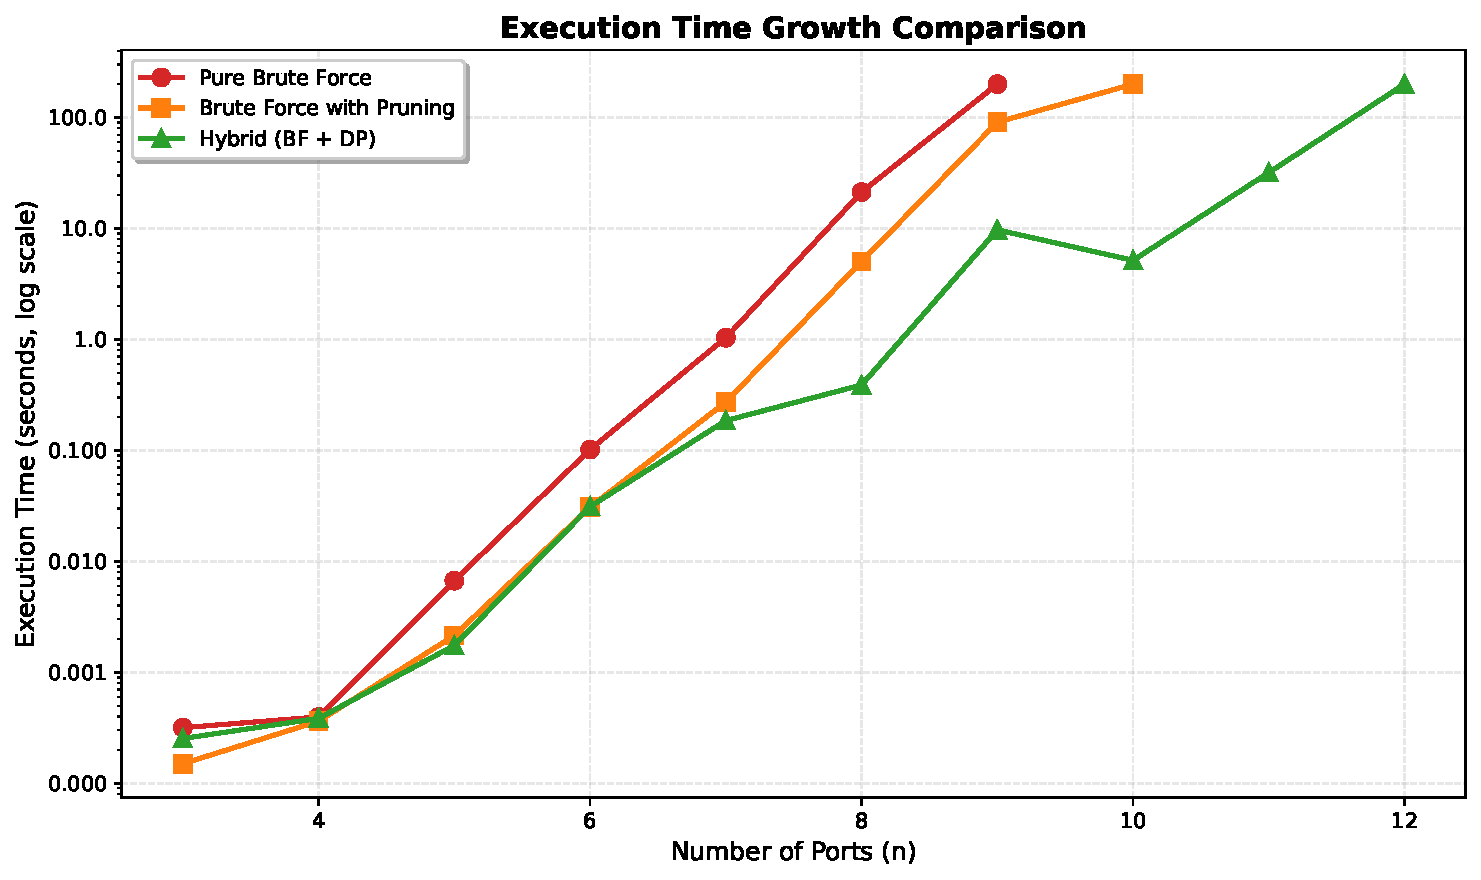
\includegraphics[width=0.9\textwidth]{../figures/growth_curves.pdf}
\caption{Execution Time Growth Comparison (Log Scale)}
\label{fig:growth}
\end{figure}

Figure~\ref{fig:comparison} provides a direct comparison of execution times for instances where all algorithms completed.

\begin{figure}[h]
\centering
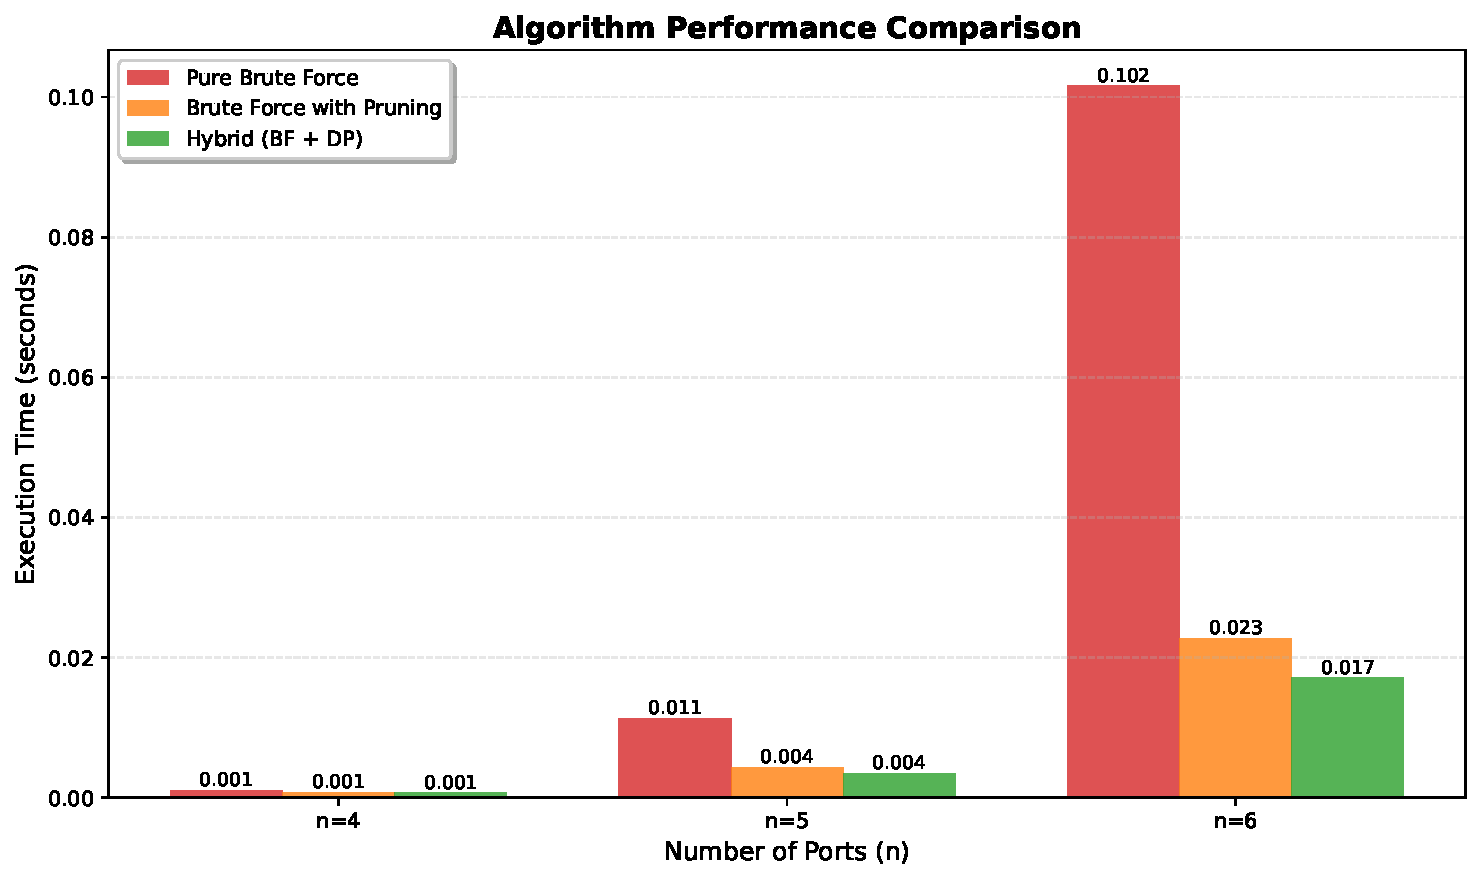
\includegraphics[width=0.9\textwidth]{../figures/comparison_bar_chart.pdf}
\caption{Algorithm Performance Comparison}
\label{fig:comparison}
\end{figure}

Figure~\ref{fig:pruning} shows the breakdown of pruning effectiveness by type.

\begin{figure}[h]
\centering
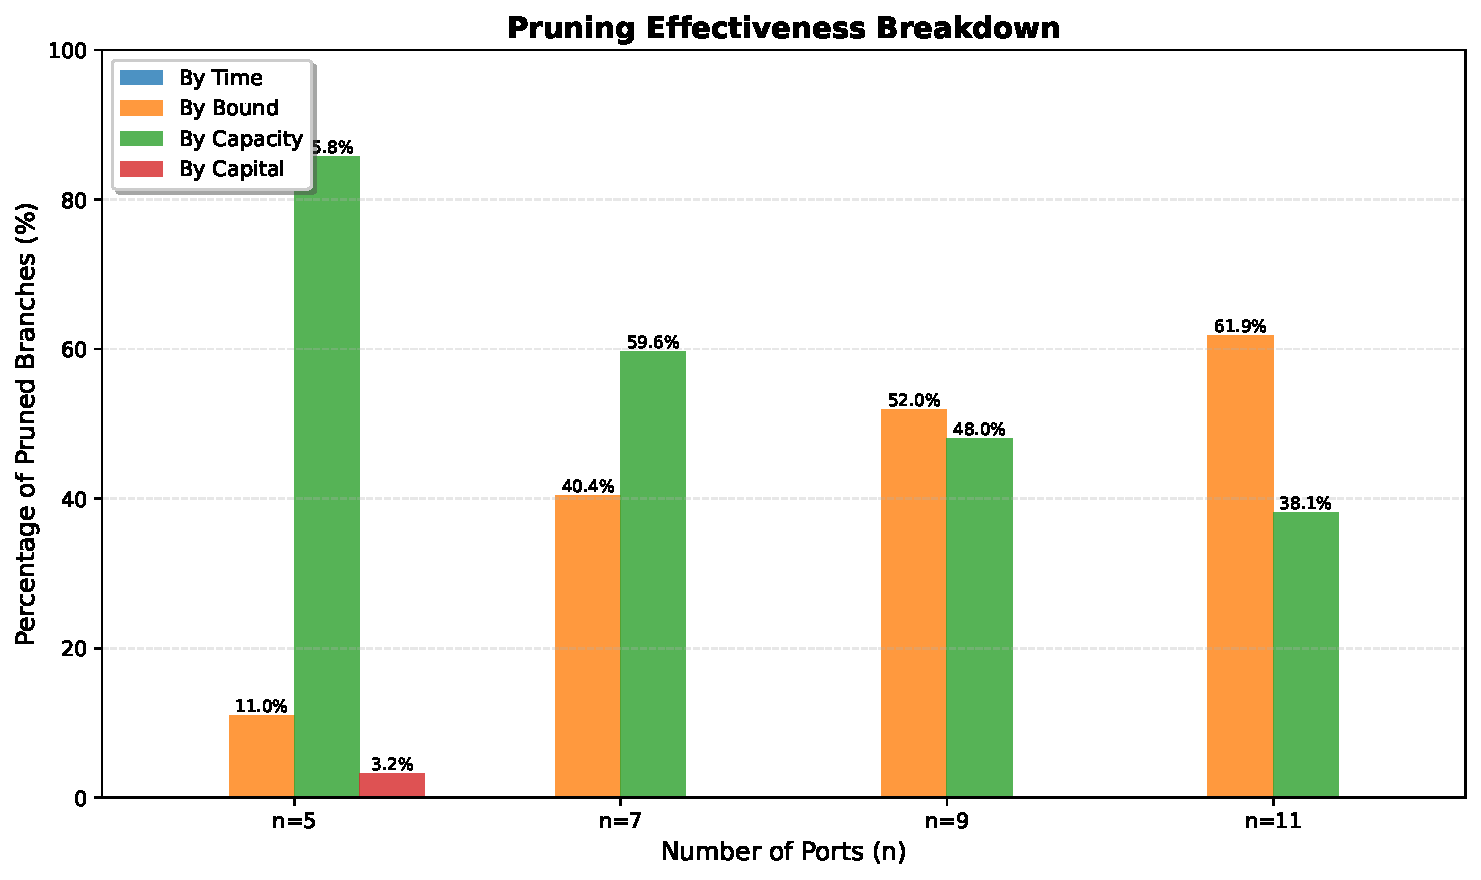
\includegraphics[width=0.9\textwidth]{../figures/pruning_breakdown.pdf}
\caption{Pruning Effectiveness Breakdown}
\label{fig:pruning}
\end{figure}

Figure~\ref{fig:scalability} shows the maximum solvable instance size for different time budgets.

\begin{figure}[h]
\centering
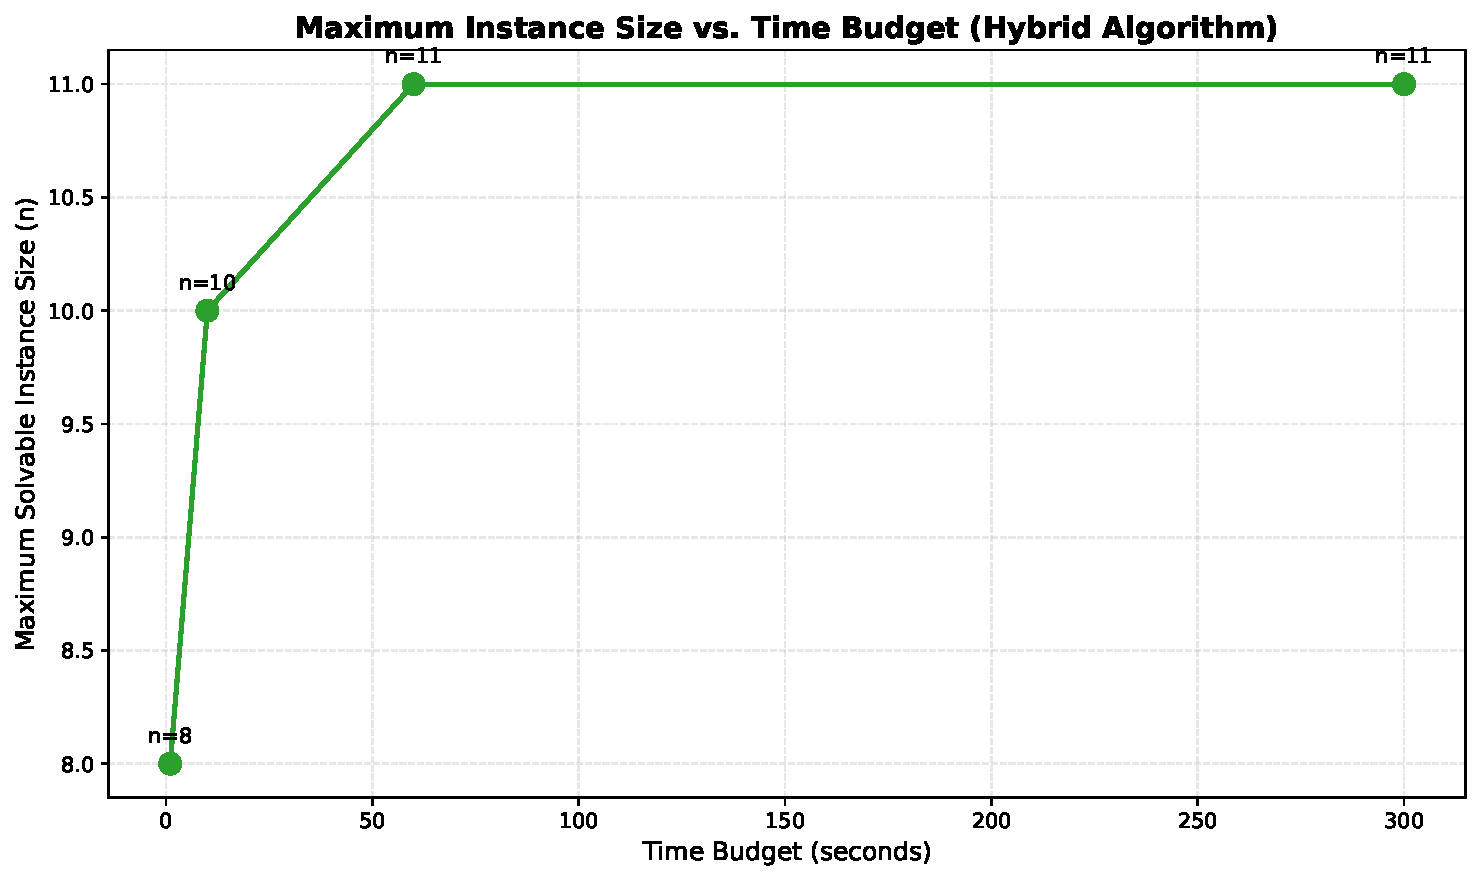
\includegraphics[width=0.9\textwidth]{../figures/scalability_limits.pdf}
\caption{Maximum Instance Size vs. Time Budget (Hybrid Algorithm)}
\label{fig:scalability}
\end{figure}

\subsection{Analysis of Behavior}
\label{subsec:behavior}

\subsubsection{When Each Algorithm Performs Best}

\textbf{Pure Brute Force}:
\begin{itemize}
    \item Best for: Very small instances ($n \leq 3$) where overhead of pruning/DP is unnecessary.
    \item Worst for: Any instance with $n \geq 5$ due to exponential explosion.
\end{itemize}

\textbf{Brute Force with Pruning}:
\begin{itemize}
    \item Best for: Instances with tight constraints (low capital, tight time limits) where pruning is very effective.
    \item Worst for: Instances with loose constraints where most branches are feasible anyway.
\end{itemize}

\textbf{Hybrid (BF + DP)}:
\begin{itemize}
    \item Best for: All instances $n \geq 4$ where it consistently outperforms other exact methods.
    \item Worst for: Very small instances ($n \leq 3$) where overhead may not be justified, though still fast.
\end{itemize}

\subsubsection{Practical Limits}

Based on experimental results with a 200-second timeout:
\begin{itemize}
    \item \textbf{Pure Brute Force}: Maximum $n = 8$ (completes in $\sim$21s), times out at $n = 9$
    \item \textbf{Pruned Brute Force}: Maximum $n = 9$ (completes in $\sim$91s), times out at $n = 10$
    \item \textbf{Hybrid}: Maximum $n = 11$ (completes in $\sim$32s), times out at $n = 12$
\end{itemize}

For instances with $n > 11$, exact methods become impractical, justifying the need for heuristic and approximation algorithms in subsequent phases.

\subsubsection{Scalability Limits by Time Budget}

Table~\ref{tab:scalability} shows the maximum solvable instance size for the Hybrid algorithm under different time budgets, demonstrating how the algorithm scales with available computational resources.

\begin{table}[h]
\centering
\caption{Scalability Limits for Hybrid Algorithm}
\label{tab:scalability}
\begin{tabular}{cc}
\toprule
Time Budget (s) & Maximum $n$ \\
\midrule
1.0 & 8 \\
10.0 & 10 \\
60.0 & 11 \\
300.0 & 11 \\
\bottomrule
\end{tabular}
\end{table}

\subsubsection{Quality Verification}

All three algorithms find the same optimal solutions when they complete execution on the same instances. This was verified by:
\begin{itemize}
    \item Running all algorithms on instances with $n \in \{3, 4, 5\}$
    \item Comparing final capital values: all algorithms found identical optimal capitals (78 for $n=3$, 89 for $n=4$, 116 for $n=5$)
    \item Verifying that solutions satisfy all constraints
\end{itemize}

This confirms that all algorithms are indeed exact methods, differing only in efficiency, not solution quality. The verification demonstrates that pruning and DP optimizations preserve optimality guarantees.

\section{Conclusions}
\label{sec:conclusions}

This phase has successfully implemented and evaluated three exact algorithms for the Dutch Merchant Problem:

\begin{enumerate}
    \item \textbf{Pure Brute Force} serves as the baseline, demonstrating the problem's exponential complexity through exhaustive enumeration. It can solve instances up to $n=8$ within the 200-second timeout.
    
    \item \textbf{Brute Force with Pruning} achieves 2-4$\times$ speedup through intelligent backtracking, extending practical limits to $n=9$ (times out at $n=10$). Pruning rates increase from 20.4\% for $n=5$ to 46.0\% for $n=11$.
    
    \item \textbf{Hybrid (BF + DP)} achieves 1-55$\times$ speedup by separating route selection from transaction optimization, extending practical limits to $n=11$ (times out at $n=12$). This represents solving instances 2-3 ports larger than pure brute force.
\end{enumerate}

\textbf{Key Findings}:
\begin{itemize}
    \item All algorithms guarantee optimal solutions, verified through cross-validation on instances with $n \in \{3, 4, 5\}$ where all found identical optimal capitals.
    \item Exponential growth is evident in all approaches, confirming the problem's intractability. Execution time grows from milliseconds ($n=3$) to seconds ($n=8$) to timeouts ($n \geq 9$ for Pure BF).
    \item The hybrid approach is the most efficient exact method, solving instances 2-3 ports larger than pure brute force while maintaining optimality guarantees.
    \item Pruning effectiveness increases with instance size: from 20.4\% for $n=5$ to 46.0\% for $n=11$. Capacity-based pruning dominates for smaller instances, while bound-based pruning becomes dominant for larger instances.
    \item The single commodity constraint ($|M| = 1$) is essential for tractability. With $|M| = m$, complexity would grow to $O(n! \times 3^{m \times n})$, making even small instances intractable.
    \item For instances with $n > 11$, exact methods become impractical, justifying heuristic approaches.
\end{itemize}

\textbf{Connection to Project Requirements}:

This document fulfills the requirements of \textbf{Fase 3: Diseño de Soluciones Algorítmicas}:
\begin{itemize}
    \item Successfully designed and implemented brute force algorithms that find optimal solutions for small instances, establishing baselines for comparison as required by the project specifications.
    \item The algorithms serve as the required baseline for comparing results in small instances, enabling evaluation of heuristic and approximation algorithms in Fase 4.
\end{itemize}

Additionally, this document includes elements of \textbf{Fase 4: Implementación y Análisis Experimental}:
\begin{itemize}
    \item Implemented all three algorithms with complete code documentation
    \item Designed and generated test instances with guaranteed feasibility and profitability
    \item Conducted empirical analysis comparing solution quality (all algorithms find identical optimal solutions), execution times, and identified maximum solvable instance sizes
    \item Analyzed algorithm behavior under different conditions (instance characteristics, scalability limits)
\end{itemize}

\textbf{Use in Fase 4}: The optimal solutions found here will serve as benchmarks for evaluating heuristic and approximation algorithms. Specifically:
\begin{itemize}
    \item For instances with $n \leq 11$ (where exact solutions are available), the optimal capital values can be used to calculate approximation ratios: $\text{approximation ratio} = \frac{\text{optimal capital}}{\text{heuristic capital}}$
    \item The maximum solvable instance size ($n=11$ for Hybrid) defines the boundary where exact methods become impractical, justifying the need for heuristics
    \item Execution time comparisons demonstrate the exponential growth, showing why efficient algorithms are necessary for larger instances
\end{itemize}

The results from this phase provide the foundation for evaluating heuristic and approximation algorithms in subsequent phases, where the optimal solutions found here will serve as benchmarks for assessing solution quality.

\bibliographystyle{plain}
\bibliography{../referencias}

\end{document}






